\documentclass{beamer}
\usepackage[utf8]{inputenc}
% \usepackage[latin1]{inputenc} %  Alternativ unter Windows
% \usepackage[T1]{fontenc}
\usepackage[ngerman]{babel}
\usepackage[toc,page]{appendix}
\usepackage{latexsym}
\usepackage{amsmath,amssymb,amsthm}
\usepackage{hyperref}

\newcommand*{\quelle}{%
	\footnotesize Quelle:
}

\useoutertheme{infolines}
\beamertemplatenavigationsymbolsempty
\setbeamertemplate{headline}{}

\title{Seminar Statistische Lernverfahren}
\subtitle{Klassifikation von Rezensionstypen}
\author[T.G., M.H., A.K., M.L., T.N., J.S.]{Till Gräfenberg, Matthias Häußler, Alexander Kohlscheen, Michael Lau, Tanja Niklas, Jonathan Schmitz}
\date{12. Dezember 2019}
\begin{document}
\begin{frame}
\thispagestyle{empty}
\titlepage
\end{frame}
%<-------------Folie 1--------->
\begin{frame}
\addtocounter{framenumber}{-1}
\frametitle{Inhaltsverzeichnis}
\begin{enumerate}\itemsep10pt
\item Problemstellung
\item Erstellen von Prädiktoren
\item Analysemethoden
	\begin{enumerate}
	\item Naive Bayes
	\item Entscheidungsbaum
	\item Random Forest
	\item Support Vector Machine
	\item weitere Anpassungen und Modelle
	\end{enumerate}
\end{enumerate}
\end{frame}
\section{Problemstellung}
\begin{frame}
\frametitle{Problemstellung}
\begin{itemize}\setlength\parskip{12pt}
\item Ziel: Klassifizierung von Reviews in folgende Typen:
\begin{center}
\begin{tabular}{c|c|c}
Texttyp & introvertiert & extrovertiert \\
\hline 
emotional & stetig & initiativ\\
rational & gewissenhaft & dominant
\end{tabular}
\end{center}
\item Gegeben: 439 bereits klassifizierte Reviews
\end{itemize}
\end{frame}


%<-------------Folie 4--------->
\section{Erstellen von Prädiktoren}
\begin{frame}
\frametitle{Erstellen von Prädiktoren}
\begin{itemize}\itemsep12pt
\item Klassifikation sollte durch verwendete Wörter geschehen
\item Zurückführung auf Grundwörter notwendig
\item Benutzung verschiedener Packages in \texttt{R} bzw. \texttt{Python} ermöglichte verschiedene Verfahren
\end{itemize}
\end{frame}

\section{Lemmatisierung und Stemming}
\begin{frame}
\frametitle{Erstellen von Prädiktoren}
\framesubtitle{Was ist Stemming?}
\begin{itemize}\setlength\parskip{12pt}
	\item Verfahren, mithilfe dessen man verschiedene Varianten eines Wortes auf ihren gemeinsamen Wortstamm zurückführt
	\item Durch Abschneiden von Prä-/In- und Suffixen und Ersetzen von Umlauten, Diphtongen etc. erzeugen von Wortstämmen
	\item Beispiele: \ \ gelernt $\rightarrow$ lernen; \ \ \ Wohnungen $\rightarrow$ Wohnung
	

\end{itemize}

\end{frame}

\begin{frame}
\frametitle{Erstellen von Prädiktoren}
\framesubtitle{Stemming}
\begin{itemize}\itemsep12pt
\item Eigene Implementierung nach Vorgabe von COMPEON in \texttt{R}
\item Für Englische Sprache bereits vorgefertigte Tools z.B. 
\begin{itemize}
\item \texttt{porterstemmer} von \texttt{nltk} in Python
\item \texttt{snowballstemmer} von \texttt{nltk} in Python
\end{itemize}
\end{itemize}

\end{frame}

\begin{frame}
\frametitle{Erstellen von Prädiktoren}
\framesubtitle{Was ist Lemmatisierung?}
\begin{itemize}
\item Das Lemma ist im Bereich der Linguistik die Grundform eines Wortes $\rightarrow$ Wortform z.B. in einem Nachschlagewerk
\item Zurückführung auf grammatikalische Grundformen
\item Lemmatisierung als ein lexikonbasiertes Stemmingverfahren
\item auftretende Probleme des Vorgangs:
\begin{itemize}
\item Ambiguitäten
\item Wahl des Lemma eines Wortes (Verbinfinitiv vs. Nomen)
\item Kompositazerlegung nicht eindeutig (Beispiel: Wachstube)
\item Simplizia (Beispiel: Kreuzer, Tangente)
\item Unregelmäßigkeit von Verben im Deutschen
\end{itemize}

\end{itemize}

\end{frame}

\begin{frame}
\frametitle{Erstellen von Prädiktoren}
\framesubtitle{Lemmatisierung}
\begin{itemize}\itemsep12pt
\item Erfordert vorgefertigte Packages z.B.
\begin{itemize}
\item \texttt{SpaCy} in Python
\item \texttt{nltk} in Python
\end{itemize}
\item Diese lieferten zusätzlich Informationen über die Wortart
\item Auch hier für Englische Sprache ausgereifter als die deutsche Alternative
\end{itemize}
\end{frame}

\begin{frame}
\frametitle{Erstellen von Prädiktoren}
\framesubtitle{Wortliste}
\begin{itemize}
\item Ausgangssituation: 439 Reviews über die Firma COMPEON 
\item 8792 Wörter in reviews\_preprocessed (mitunter mehrfach)
\end{itemize}
\begin{table}
	\centering
		\begin{tabular}[h]{l|c|r}
			cleaned\_text & preprocessed\_text \\
			\hline
			richtigen & richtig \\
			\hline
			darlehen & darleh \\
			\hline
			gewünschte & wunsch \\
			\hline
			taggenuae & taggenua \\
			\hline
			gegenüber & genub
			
			
		\end{tabular}
		\item
	\caption{Wortliste Beispiele}
	\label{tab:WortlisteBeispiele}
\end{table}
\end{frame}

\begin{frame}
\frametitle{Erstellen von Prädiktoren}
\framesubtitle{Filterung der Prädiktoren}
\begin{itemize}\itemsep12pt
\item Nach Erstellung der Grundwörter konnte gefiltert werden, welche Wörter häufig auftraten
\item Denkbare Filtermethoden für das Wörterbuch:
\begin{itemize}
\item Nur Wörter, die mind. $n$ Mal aufgetaucht sind 
\item Nur Wörter, die in mind. $p\%$ der Reviews verwendet wurden
\end{itemize} 
\item Anschließend Erstellung einer binären Document-Term-Matrix, die kodiert, welche Grundwörter in welchen Reviews auftauchten
\item Alternative: PCA um aussagekräftige \glqq Wörterachsen\grqq \,zu bestimmen. Kein sichtbarer Erfolg.
\end{itemize}
\end{frame}

\begin{frame}
\frametitle{Erstellen von Prädiktoren}
\framesubtitle{Document-Term-Matrix}
\begin{itemize}\itemsep12pt
\item Wörterbucherstellung aus den verbliebenen Grundwörtern\\
\begin{center}
\begin{tabular}{|c|c|c|c|c|}
\hline
		& Lemma 	& n	\\
\hline
144 	& .		& 654\\
143	 	& der	& 531\\
142 	& und	& 440\\
%141	 	& ,		& 413\\
%140	 	& ich	& 318\\
...		& ...	& ...\\
2		& dann & 10\\
1		& abschluss & 10\\
\hline
\end{tabular}
 \end{center}

%\item Erstellung der DTM unter Beachtung der numerischen Reihenfolge der $doc\_id$s (d.h. nicht alphabetisch)
\item DTM-Zeilen: Reviews 1 bis 439, DTM-Spalten: Grundwörter aus Wörterbuch
\item zusätzliche Spalten: doc\_id, review, type (Zielvariable) 
\item Kodierung: Wort kommt in der Review vor (1) oder nicht (0)
\end{itemize}
\end{frame}

\begin{frame}
\frametitle{Erstellen von Prädiktoren}
\framesubtitle{Document-Term-Matrix}
\begin{itemize}\itemsep12pt
\item Anfügen weiterer Prädiktoren mit Anzahlen pro Review der
\begin{itemize}
\item Wörter %$count\_of\_words$
\item Fragen %$count\_of\_questions$
\item Imperative %$count\_of\_imperatives$
\item Sätze %$count\_of\_sentences$
\item Nebensätze/Trennungen %$count\_of\_subordinated\_clauses\_and\_separations$
\item Satzzeichen %$count\_of\_punctuation$
(ggf. einzeln betrachtet)
\item Wortarten %$count\_of\_parts\_of\_speech$
\end{itemize} 
\item Weitere Variablenselektion möglich

\end{itemize}
\end{frame}

\begin{frame}
\frametitle{Erstellen von Prädiktoren}
\framesubtitle{Document-Term-Matrix}
\vspace{12pt}
\begin{tabular}{|c|c|c|c|c|c|c|c|c|c|}
\hline
...	&dass&  der 	& dies & ... & doc\_id	& review & words & ...& type\\
\hline
... &0& 1		& 0		&	...	& 1		& Die Un...&12 			& ...& Ge\\
...	& 0&0		& 0		&	...	& 2		& schnell...&7 			& ...& In\\
...	& 0&0		& 0		&	...	& 3		& Sehr g...&9 			& ...& Do\\
...	& 0&0		& 0		&	...	& 4		& Super ...&8 			& ...& In\\
...	& 0&1		& 0		&	...	& 5		& Hervor...&11 			& ...& In\\
...	& 0&1		& 0		&	...& 6		& Die Zu...&27 			& ...& In\\
...	& 0&1		& 0		&	...& 7		& untern...&26 			& ...& In\\
...	& 0&1		& 0		&	...& 8		& Schnell...&23 			& ...& Ge\\
...	& 0&0		& 0		&	...& 9		& Unkom...&3 			& ...& Do\\
...	& 0&1		& 0		&	...& 10	& ich ha...&39 			& ...& St\\
...	& 0&1		& 0		&	...	& 11	& Besten...&19 			& ...& St\\
...	& 0&0		& 0		&...	& 12	& Sehr f...&8 			& ...& In\\
...	& ...&...	&...	&	...	& ...  	& ...		&... 			& ...& ...\\
\hline
\end{tabular}


%\begin{center}
%	\includegraphics[scale=0.5]{DFGHJKLKJHGFFKLKJHGFDFZULKJHGFDFGHJKLKJHGF.png}
%\end{center}
\end{frame}


\section{Analysemethoden}
\subsection{Lineare Modelle}
\begin{frame}
\frametitle{Analysemethoden}
\framesubtitle{Lineare Modelle}
\begin{itemize}\itemsep12pt
\item Idee: Vorhersagen der Labels in Form eines linearen Zusammenhangs 
\begin{align*}
y=\beta^T\cdot x+\epsilon
\end{align*}
mit $\epsilon~\raisebox{-0.9ex}{\~{ }} ~ \mathcal{N}_{n}(0,\sigma)$ und $\beta=(X^TX)^{-1}Xy$;\\
die Zeilen der DTM entsprechen unserem $x$ 
\item Da das Modell eine Zahl zurückgibt, müssen die einzelnen Typen oder alternativ die Eigenschaften extro-/introvertiert bzw. emotional/rational separat betrachtet werden.
\end{itemize}
\end{frame}

\begin{frame}
\section{Analysemethoden}
\subsection{Lineare Modelle}
Lineares Modell, \texttt{R}, Wortaufkommen $\geq$ 20\\
%Mit einem linearen Modell und der Typisierung in dominant gewissenhaft initiativ oder stetig als zusätzlichen Prädiktor lässt sich nicht zuverlässig klassifizieren:\\
\vspace{12pt}
\begin{tabular}{|c|c|c|c|c|c|c|c|c|}
\hline
				& D 	& G	& I & S	& Acc.	& Prec. & Recall	& F1\\
\hline
Dominant 		& 11	& 2 & 12& 5 &      	& 0,367 & 0,611 	& 0,458\\
Gewissenhaft 	& 4 	& 5 & 12& 4 & 		& 0,200 & 0,357 	& 0,256\\
Initiativ 		& 2 	& 4	& 11& 7	& 		& 0,458	& 0,306 	& 0,367\\
Stetig 			& 1 	& 3 & 1 & 2 & 		& 0,286	& 0,111 	& 0,160\\
\hline
Total 			& 		& 	& 	& 	& 0,337	& 0,328 & 0,346  	& 0,310\\
\hline
\end{tabular}
\end{frame}

\begin{frame}
\section{Analysemethoden}
\subsection{Lineare Modelle}
Lineares Modell, \texttt{R}, Wortaufkommen $\geq$ 20\\
%Mit linearen Modellen und jeweils nur der Klassifizierung nach extro-/introvertiert bzw. emotional/rational als zusätzlichen Prädiktor lässt sich jeweils zuverlässig klassifizieren:\\
\vspace{12pt}
\begin{center}
\begin{tabular}{|c|c|c|c|c|c|c|c|c|}
\hline
				& emotional 	& rational	&  Acc.	& Prec. & Recall	& F1\\
\hline
emotional 		& 24			& 19 		&       & 0,558	& 0,750 	& 0,640\\
rational	 	& 8 			& 35		& 		& 0,814	& 0,648 	& 0,722\\
\hline
Total 			& 				& 			& 0,686	& 0,343	& 0,350  	& 0,340\\
\hline
\end{tabular}
\end{center}

\begin{center}
\begin{tabular}{|c|c|c|c|c|c|c|c|c|}
\hline
				& extro. 	& intro.	&  Acc.	& Prec. 	& Recall	& F1\\
\hline
extrovertiert	& 43		& 20		&       & 0,683 	& 0,796 	& 0,735\\
introvertiert 	& 11 		& 12		& 		& 0,522 	& 0,375 	& 0,436\\
\hline
Total 			& 			& 			& 0,640	& 0,301		& 0,293  	& 0,293\\
\hline
\end{tabular}
 \end{center}

 \vspace{12pt}
 
 Idee:\\
 Nutze die Vorhersage dieses Modells, um ein neues Modell anzupassen. 
 \end{frame}

\begin{frame}
\section{Analysemethoden}
\subsection{Lineare Modelle}
Modifiziertes Modell aus beiden vorherigen linearen Modellen, \texttt{R}, Wortaufkommen $\geq$ 20\\
%Mit der Kombination aus den beiden vorherigen linearen Modellen (also unter separater Betrachtung der Klassifizierungen nach extro-/introvertiert und emotional/rational) lässt sich zuverlässiger klassifizieren:\\
\vspace{12pt}
\begin{tabular}{|c|c|c|c|c|c|c|c|c|}
\hline
				& D 	& G	& I & S	& Acc.	& Prec. & Recall	& F1\\
\hline
Dominant 		& 13	& 4 & 12& 2 &      	& 0,419 & 0,722 	& 0,531\\
Gewissenhaft 	& 2 	& 5 & 4 & 1 & 		& 0,417 & 0,357 	& 0,385\\
Initiativ 		& 2 	& 3	& 16& 11& 		& 0,500	& 0,444 	& 0,471\\
Stetig 			& 1 	& 2 & 4	& 4 & 		& 0,364	& 0,222 	& 0,276\\
\hline
Total 			& 		& 	& 	& 	& 0,442	& 0,425 & 0,437	  	& 0,415\\
\hline
\end{tabular}
 \vspace{12pt}
 
Das modifizierte Modell liefert eine höhere Zuverlässigkeit.
\end{frame}


\begin{frame}
 \frametitle{Erstellen von Prädiktoren}
 \framesubtitle{PCA - Principal Component Analysis}
 Ziel: Dimensionsreduktion \\
 \vspace{12pt}
 Idee: Suche die Datenachsen, auf denen die Varianz am größten ist \\
 \vspace{12pt}
 Verfahren:\\
 
 \begin{itemize}
  \item Sei $X$ die DT-Matrix (Spaltenmittelwerte = 0)
  \item Bestimme die Kovarianzmatrix $Cov = X^TX$
  \item Bestimme die Eigenwerte $\lambda_i$ und Eigenvektoren $v_i$ von $Cov$
  \item Sei $V = (v_1| v_2| ...)$
  \item Transformiere die Daten zu $\hat{X} = X V$
 \end{itemize}

 \vspace{12pt}
 Problem: Die Resultate verlieren an Interpretierbarkeit
 
\end{frame}

\begin{frame}
 \frametitle{Erstellen von Prädiktoren}
 \framesubtitle{PCA - Principal Component Analysis}
 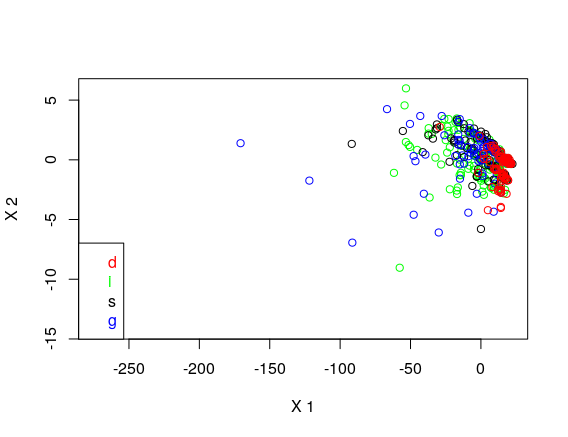
\includegraphics[scale=0.36]{PCA_1_2.png}
 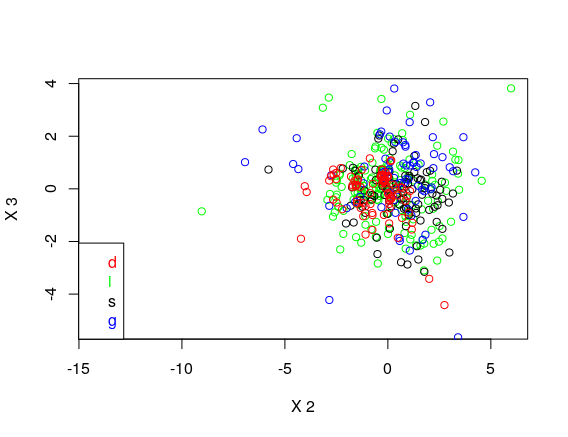
\includegraphics[scale=0.36]{PCA_2_3.png}
 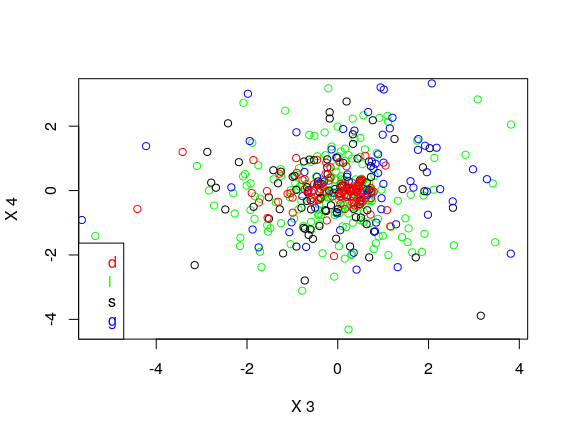
\includegraphics[scale=0.36]{PCA_3_4.png}
 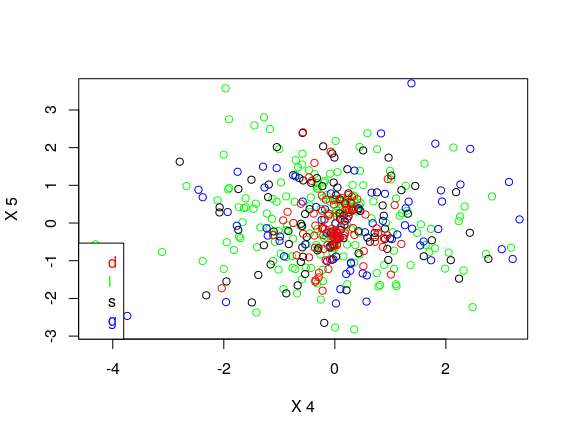
\includegraphics[scale=0.36]{PCA_4_5.png}
 
\end{frame}

\begin{frame}
 \frametitle{Erstellen von Prädiktoren}
 \framesubtitle{PCA - Principal Component Analysis}
 Fazit:
 \begin{itemize}
  \item Die Dominanten Reviews haben eine geringere Varianz
  \item keine erkennbaren Gruppen
  \item Mittelwerte der Gruppen sind ähnlich
 \end{itemize}
 
 Das Verfahren liefert keine besseren Ergebnisse und benötigt nicht wesentlich weniger Variablen. 

\end{frame}

\subsection{Naive Bayes}
%<-------------Folie 8--------->

% Jonathans Text
\begin{frame}
\frametitle{Analysemethoden}
\framesubtitle{Naive Bayes}
\begin{itemize}\itemsep12pt
\item Das Naive Bayes Verfahren fußt auf dem Bayes Theorem
\[p(y|x) = \frac{p(x|y)p(y)}{p(x)}\]
bzw. für unabhängige Prädiktoren $x_1,...,x_n$ als
\[p(y|x_1,...,x_n)=\frac{p(x_1|y)\cdots p(x_n|y)p(y)}{p(x_1,...,x_n)}\propto p(x_1|y)\cdots p(x_n|y)p(y).\]
\item Durch Schätzen von $p(y)$ und $p(x_i|y)$ (für die Reviewtypen $y$) durch die relativen Häufigkeiten, können wir dann Klassifikationen durchführen als
\[\hat{y}=\text{argmax}_y\,p(y)\prod_{i=1}^np(x_i|y).\]
\end{itemize}
\end{frame}

\begin{frame}
\frametitle{Analysemethoden}
\framesubtitle{Naive Bayes}
\begin{itemize}\itemsep12pt
\item Durchführung war in \texttt{R} mit dem Package \texttt{caret}, über \texttt{Python} mit \texttt{sklearn} möglich. Mit letzterem haben wir jeweils die deutschen und englischen Reviews klassifiziert.
\item Dieses Vorgehen zeigte nur wenig bessere Ergebnisse als eine einheitliche Zuweisung.
\end{itemize}
\begin{center}
(Bester) Naive Bayes, \texttt{R}, Wortaufkommen $> 20$\
\begin{tabular}{|c|c|c|c|c|c|c|c|c|}
\hline
				& D 	& G	& I & S	& Acc.	& Prec. & Recall	& F1\\
\hline
Dominant 		& 14		& 2 			& 8 		& 1 		&       	& 0,412 	& 0,778 	& 0,538\\
Gewissenhaft 	& 0 		& 0 			& 0 		& 0 		& 			& n.d. 		& 0 	& n.d.\\
Initiativ 		& 4 		& 11			& 28		& 17		& 			& 0,467	& 0,778 	& 0,583\\
Stetig 			& 0 		& 1 			& 0 		& 0 		& 			& n.d.	   		& 0 	& n.d\\
\hline
Total 			& 			& 				& 			& 			& 0,494		& n.d. 		& 0,389  	& n.d.\\
\hline
\end{tabular}
\end{center}
\end{frame}

\begin{frame}
\begin{center}
Naive Bayes, \texttt{Python}, Wortvorkommen in mind. 1\% der Texte,\\
Lemmatisierung mit spacy, Englisch\
\begin{tabular}{|c|c|c|c|c|c|c|c|c|}
\hline
 & D 	& G	& I & S	& Acc.	& Prec. & Recall	& F1\\
\hline
Dominant & 13 & 4 & 12 & 4 & & 0,433 & 0,722 & 0,542\\
Gewissenhaft & 0 & 3 & 3 & 0 & & 0,5 & 0,214 & 0,3\\
Initiativ & 4 & 5 & 16 & 11 & & 0,444 & 0,444 & 0,444\\
Stetig & 1 & 2 & 5 & 3 & & 0,273 & 0,167 & 0,207\\
\hline
Total  &   &   &   &   & 0,407 & 0,413  & 0,387   & 0,373\\
\hline
\end{tabular}
\end{center}
\end{frame}

\begin{frame}
\begin{center}
Naive Bayes, \texttt{Python}, Wortvorkommen in mind. 1\% der Texte,\\
Lemmatisierung mit spacy, Deutsch\
\begin{tabular}{|c|c|c|c|c|c|c|c|c|}
\hline
 & D 	& G	& I & S	& Acc.	& Prec. & Recall	& F1\\
\hline
Dominant & 16 & 2 & 13 & 2 & & 0,444 & 0,889 & 0,593\\
Gewissenhaft & 0 & 5 & 4 & 1 & & 0,5 & 0,357 & 0,417\\
Initiativ & 2 & 5 & 16 & 13& & 0,444 & 0,444 & 0,444\\
Stetig & 0 & 2 & 3 & 2& & 0,286 & 0,111 & 0,16 \\
\hline
Total  &   &   &   &   & 0,453 & 0,419  & 0,45   & 0,403\\
\hline
\end{tabular}
\end{center}
\end{frame}

\subsection{Weitere Methoden}
\begin{frame}
 \frametitle{Analysemethoden}
 \framesubtitle{weitere Anpassungen und Modelle}
 Mit Naive Bayes und den Wortarten als Prädiktoren lässt sich zuverlässig voraussagen,
 ob eine Person extrovertiert ist:\\
 \vspace{12pt}
 \begin{center} 
 Naive Bayes, \texttt{R}, Wortarten, Wortvorkommen in mind. 10 Texten
  \begin{tabular}{c|c|c|c|c|c|c|}
                & extro & intro & Acc.  & Prec. & Recall    & F1 \\
  \hline
  extrovertiert & 30    & 5     &       & 0,714 & 0,556     & 0,625 \\
  introvertiert & 24    & 27    &       & 0,529 & 0,843     & 0,65 \\
  \hline
  Total         &       &       & 0,663 & 0,622 & 0,7       & 0,638 \\
  \hline
 \end{tabular}
 
 \end{center}

 \vspace{12pt}
 
 Idee:\\
 Nutze die Vorhersage dieses Modells um ein neues Modell anzupassen.
\end{frame}

\begin{frame}
 \frametitle{Analysemethoden}
 \framesubtitle{weitere Anpassungen und Modelle}
 
 Random Forest, \texttt{R}, Wortvorkommen in mind. 10 Texten
 \begin{center}
 \begin{tabular}{c|c|c|c|c|c|c|c|c|}
                & D     & G  & I    & S   & Acc.  & Prec. & Recall    & F1 \\
  \hline
  Dominant      & 14    & 2  & 8    & 1   &       & 0,56  & 0,778     & 0,561 \\
  Gewissenhaft  & 1     & 4  & 1    & 0   &       & 0,667 & 0,286     & 0,4 \\
  Initiativ     & 3     & 7  & 25   & 15  &       & 0,5   & 0,694     & 0,581\\
  Stetig        & 0     & 1  & 2    & 2   &       & 0,4   & 0,111     & 0,174\\
  \hline
  Total         &       &    &      &     & 0,523 & 0,532 & 0,467     & 0,452\\
  \hline
 \end{tabular}
 \end{center}
 
 \vspace{12pt}
 Random Forest mit Naive Bayes, \texttt{R}, Wortvorkommen in mind. 10 Texten
 \begin{center}
  \begin{tabular}{c|c|c|c|c|c|c|c|c|}
                & D     & G  & I    & S   & Acc.  & Prec. & Recall    & F1 \\
  \hline
  Dominant      & 15    & 2  & 9    & 1   &       & 0,577 & 0,833     & 0,682 \\
  Gewissenhaft  & 0     & 4  & 1    & 1   &       & 0,667 & 0,286     & 0,4 \\
  Initiativ     & 3     & 8  & 24   & 13  &       & 0,5   & 0,667     & 0,571\\
  Stetig        & 0     & 0  & 2    & 3   &       & 0,6   & 0,167     & 0,261\\
  \hline
  Total         &       &    &      &     & 0,535 & 0,586 & 0,488     & 0,479\\
  \hline
 \end{tabular}
 \end{center}
 
\end{frame}

 % Matthias Text
\subsection{Entscheidungsbaum}
\begin{frame}
\frametitle{Analysemethoden}
\framesubtitle{Entscheidungsbaum}
\begin{itemize}\setlength\parskip{12pt}
\item Teilt in Klassen auf
\item Wahr- oder Falsch-Entscheidungen
\item Jedes Blatt hat genau eine Klasse
\item Verwende \texttt{rpart}
\end{itemize}
\end{frame}

\begin{frame}
\frametitle{Analysemethoden}
\framesubtitle{Entscheidungsbaum}
\begin{center}
	\includegraphics[scale=0.5]{RPlot.pdf}
\end{center}

\end{frame}
%<-------------Folie--------->
\begin{frame}
\frametitle{Analysemethoden}
\framesubtitle{Entscheidungsbaum}
Resultate Entscheidungsbaum, \texttt{R}, Wortaufkommen $> 20$
\begin{center}
\begin{tabular}{|c|c|c|c|c|c|c|c|c|}
\hline
 &  D 	& G	& I & S	& Acc.	& Prec. & Recall	& F1\\
\hline
Dominant & 14 & 3 & 9 & 1 & & 0.518 & 0.777 & 0.621 \\
Gewissenhaft & 0 & 3 & 5 & 5& &0.23 & 0.21,4 & 0.221\\
Initiativ & 2 & 4 & 19 & 5& & 0.633& 0.527 & 0.575\\
Stetig & 2 & 4 & 3 & 7& &0.437 & 0.388& 0.411 \\
\hline
Total 	&		&		& & 		& 0.5	& 0.454& 0.476 & 0.454\\
\hline
\end{tabular}
\end{center}
\end{frame}
%<-------------Folie--------->
\begin{frame}
\frametitle{Analysemethoden}
\framesubtitle{Entscheidungsbaum}
Resultate Entscheidungsbaum, \texttt{Python}, mind. in 1\% der Texte, Englisch
\begin{center}
\begin{tabular}{|c|c|c|c|c|c|c|c|c|}
\hline
 &  D 	& G	& I & S	& Acc.	& Prec. & Recall	& F1\\
\hline
Dominant &     9 & 4 & 12 & 5& &0.3 & 0.5 & 0.375 \\
Gewissenhaft & 2 & 3 & 4 & 2&& 0.272 & 0.214 & 0.239 \\
Initiativ &    5 & 5 & 12 & 8&& 0.4 & 0.333 & 0.363\\
Stetig &       2 & 2 & 8 & 3&& 0.2 & 0.166& 0.181 \\
\hline
Total 	&		&		& &	& 0.313		& 0.293 & 0.303 & 0.289 \\
\hline
\end{tabular}
\end{center}
\end{frame}
%<-------------Folie--------->
\begin{frame}
\frametitle{Analysemethoden}
\framesubtitle{Entscheidungsbaum}
Resultate Entscheidungsbaum, \texttt{Python}, mind. in 1\% der Texte, Deutsch
\begin{center}
\begin{tabular}{|c|c|c|c|c|c|c|c|c|}
\hline
 &  D 	& G	& I & S	& Acc.	& Prec. & Recall	& F1\\
\hline
Dominant &     13 & 4 & 16 & 1&&  0.382 & 0.722 & 0.499 \\
Gewissenhaft & 2 & 4 & 1 & 3 &&  0.4 & 0.285 & 0.332  \\
Initiativ &    3 & 5 & 13 & 7&& 0.464 & 0.361 & 0.406  \\
Stetig &       0 & 1 & 6 & 7 &&  0.5 & 0.388 & 0.436 \\
\hline
Total 	&		&		& & 		&  0.430			&  0.436 &0.439 & 0.418 \\
\hline
\end{tabular}
\end{center}
\end{frame}
%<-------------Folie--------->
\subsection{Random Forest}
\begin{frame}
\frametitle{Analysemethoden}
\framesubtitle{Random Forest}
\begin{itemize}\setlength\parskip{12pt}
\item Entscheidungsbaum nicht beste Option
\begin{itemize}
	\item Gut für Trainingsdaten
	\item Nicht flexibel 
	\item Probleme mit neuen Datensätzen
\end{itemize}
\item Generiere neue Testdaten durch Wählen mit Zurücklegen
\item Erzeuge Entscheidungsbaum
\item Generiere so viele Entscheidungsbäume
\item Entscheidung durch Mehrheitsentscheidung
\item \texttt{R} \texttt{randomForest} 2000 Bäume, analog in  \texttt{Python}
\end{itemize}
\end{frame}
%<-------------Folie--------->
\begin{frame}
\frametitle{Analysemethoden}
\framesubtitle{Random Forest}
Resultate Random Forest, \texttt{R}, Wortaufkommen $> 20$
\begin{center}
\begin{tabular}{|c|c|c|c|c|c|c|c|c|}
\hline
 &  D 	& G	& I & S	& Acc.	& Prec. & Recall	& F1\\
\hline
Dominant & 14 & 2 & 10& 0 &&0.538 & 0.777 & 0.635 \\
Gewissenhaft & 2 & 4 & 0 & 1&&0.571 & 0.285 & 0.28 \\
Initiativ & 2 & 7  & 25 & 14&&0.52 & 0.694 & 0.594 \\
Stetig & 0 & 1 & 1 &  3&&0.6 & 10.66 & 0.26 \\
\hline
Total 	&		&		& & 		& 0.534		&   0.557 & 0.48 & 0.442\\
\hline
\end{tabular}
\end{center}
\end{frame}
%<-------------Folie--------->
\begin{frame}
\frametitle{Analysemethoden}
\framesubtitle{Random Forest}
Resultate Random Forest, \texttt{Python}, mind. in 1\% der Texte, Englisch
\begin{center}
\begin{tabular}{|c|c|c|c|c|c|c|c|c|}
\hline
 &  D 	& G	& I & S	& Acc.	& Prec. & Recall	& F1\\
\hline
Dominant & 16 & 4 & 14 & 4 &&0.421 & 0.888 & 0.571 \\
Gewissenhaft & 0 & 6 & 2 & 1&&0.666 & 0.428 & 0.521 \\
Initiativ & 1 & 4 & 16 & 9&&0.533 & 0.444 & 0.484 \\
Stetig & 1 & 0 & 4 & 4&&0.444 & 0.222 & 0.296 \\
\hline
Total 	&		&		& & 		& 0.488		&  0.516 & 0.495 & 0.468\\
\hline
\end{tabular}
\end{center}
\end{frame}
%<-------------Folie--------->
\begin{frame}
\frametitle{Analysemethoden}
\framesubtitle{Random Forest}
Resultate Random Forest, \texttt{Python}, mind. in 1\% der Texte, Deutsch
\begin{center}
\begin{tabular}{|c|c|c|c|c|c|c|c|c|}
\hline
 &  D 	& G	& I & S	& Acc.	& Prec. & Recall	& F1\\
\hline
Dominant & 15 & 4 & 15 & 2 &&0.416 & 0.833 & 0.554 \\
Gewissenhaft & 0 & 3 & 4 & 3&&0.3 & 0.214 & 0.249 \\
Initiativ & 2 & 4 & 15 & 9&&0.5 &0.416 & 0.454 \\
Stetig & 1 & 3 & 2 & 4&&0.4 & 0.222 & 0.285 \\
\hline
Total 	&		&		& & 		& 0.43		&    0.404 & 0.421 & 0.385\\
\hline
\end{tabular}
\end{center}
\end{frame}

% Michaels Text
\subsection{Support Vector Machine}
\begin{frame}
\frametitle{Analysemethoden}
\framesubtitle{Support Vector Machine}
\begin{itemize}\setlength\parskip{12pt}
\item Versucht Entscheidungsgrenze (Hyperebene) zu finden, die die Distanz der nächsten Datenpunkte jeder Klasse zu ihr maximiert
\item Diese nächsten Datenpunkte sind die \textit{Support Vectors}
\end{itemize}
\begin{figure}
	\centering
	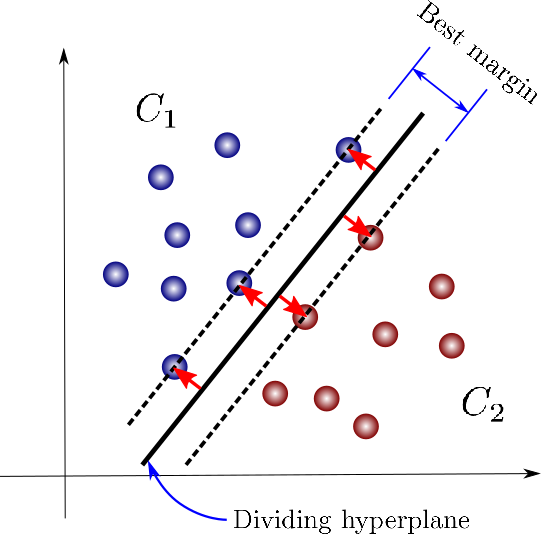
\includegraphics[scale=0.25]{svm.png}\\
	\quelle\url{https://towardsdatascience.com/support-vector-machines-for-classification-fc7c1565e3}
\end{figure}
\end{frame}
%<-------------Folie--------->
\begin{frame}
\frametitle{Analysemethoden}
\framesubtitle{Support Vector Machine}
\begin{itemize}\setlength\parskip{12pt}
	\item Verschiedene Kerne (Funktionen) um dem Separierungsproblem gerecht zu werden
	\item Kerne projizieren nicht-linear separierbare Daten niedrigerer Dimensionen auf linear-separierbare Daten höherer Dimensionen
	\item Vier häufig verwendete Kerne:
	\begin{itemize}
		\item \makebox[3.1cm][l]{Linear} $\langle u, v \rangle$
		\item \makebox[3.1cm][l]{Polynomiell} $(\gamma \langle u, v \rangle + r)^d$
		\item \makebox[3.1cm][l]{Radial} $\exp(-\gamma \| u-v \|^2)$
		\item \makebox[3.1cm][l]{Sigmoidal} $\tanh(\gamma \langle u,v \rangle + r)$
	\end{itemize}
	\item In \texttt{R} mit \texttt{e1071} und in Python mit \texttt{sklearn}
\end{itemize}
\end{frame}
%<-------------Folie--------->
\begin{frame}
\frametitle{Resultate Support Vector Machine}
\begin{center}
Support Vector Machine, \texttt{R}, Wortvorkommen mind. 10 mal,\\
Radialer Kern, Modifizierter CISTEM-Stemmer, Deutsch

\bigskip

\begin{tabular}{|c|c|c|c|c|c|c|c|c|}
\hline
				& D 	& G	& I & S	& Acc.	& Prec. & Recall	& F1\\
\hline
Dominant 		& 14		& 3 			& 8 		& 1 		&       	& 53,8\% 	& 77,8\% 	& 63,6\%\\
Gewissenhaft 	& 0 		& 1 			& 1 		& 0 		& 			& 50,0\% 	& 7,1\% 	& 16,3\%\\
Initiativ 		& 4 		& 10			& 27		& 14		& 			& 57,0\%		& 75,0\% 	& 41,9\%\\
Stetig 			& 0 		& 0 			& 0 		& 3 		& 			& 100\%	   	& 16,7\% 	& 20,9\%\\
\hline
Total 			& 			& 				& 			& 			& 52,33\%	& 63,2\%		& 44,1\%  	& 41,0\%\\
\hline
\end{tabular}
\end{center}
\end{frame}
%<-------------Folie--------->
\begin{frame}
\frametitle{Resultate Support Vector Machine}
\begin{center}
Support Vector Machine, \texttt{Python}, Wortvorkommen mind. 20 mal,\\
Sigmoid Kern, Porter-Stemmer aus \texttt{nltk}, Englisch

\bigskip

\begin{tabular}{|c|c|c|c|c|c|c|c|c|}
\hline
				& D 	& G	& I & S	& Acc.	& Prec. & Recall	& F1\\
\hline
Dominant 		& 14		& 2 			& 9 		& 1 		&       	& 54\%	 	& 78\%	 	& 64\%\\
Gewissenhaft 	& 0 		& 5 			& 4 		& 1 		& 			& 50\%	 	& 36\%	 	& 42\%\\
Initiativ 		& 3 		& 5				& 19		& 13		& 			& 47\%		& 53\%	 	& 50\%\\
Stetig 			& 1 		& 2 			& 4 		& 3 		& 			& 30\%	   	& 17\%	 	& 21\%\\
\hline
Total 			& 			& 				& 			& 			& 47,7\%		& 45\%		& 46\%  	& 44\%\\
\hline
\end{tabular}
\end{center}
\end{frame}
%<-------------Folie--------->
\subsection{Schwierigkeiten}
\begin{frame}
\frametitle{Schwierigkeiten}
\begin{itemize}
	\item Keine eindeutige Klassifikation
	\begin{itemize}
		\item Auch für Menschen nicht eindeutig
		\item Teilweise sehr geringe Unterschiede zwischen den Typen
	\end{itemize}
	\item Stemming nicht unbedingt eindeutig
	\begin{itemize}
		\item Unregelmäßigkeit von Verben im Deutschen
		\item Komposita
	\end{itemize}
	\item Geringe Zahl an Trainingsdaten
	\item Unbalanciertes Studiendesign
	\item Representativität
	\begin{itemize}
		\item Introvertierte Kunden schreiben weniger häufig Reviews
		\item Nur positive Bewertungen lagen vor
	\end{itemize}
\end{itemize}
\end{frame}

\end{document}
